\begin{frame}{POSIX error handling}
\begin{itemize}
\item most commonly POSIX functions return -1 on error
    \begin{itemize}
    \item some exceptions; check \texttt{man function\_name}
    \end{itemize}
\item usually set variable \texttt{errno}
    \begin{itemize}
    \item what went wrong?
    \end{itemize}
\item tools for using \texttt{errno}
    \begin{itemize}
    \item \texttt{strerror(errno)} --- human-readable error string
    \item \texttt{perror("name")} --- print `name: \textit{error}' to stderr
    \end{itemize}
\end{itemize}
\end{frame}

\begin{frame}{error lists}
\begin{itemize}
\item from \texttt{man fork} on Linux
    \begin{itemize}
    \item possible errors are E\textit{SOMETHING} constants declared in \texttt{errno.h}
    \end{itemize}
\end{itemize}
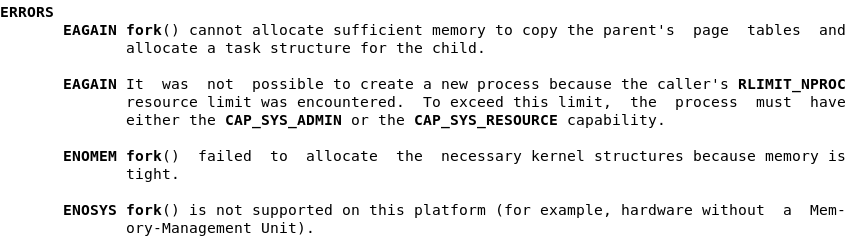
\includegraphics[width=0.99\textwidth]{../unix-api/fork-errors}
\end{frame}
